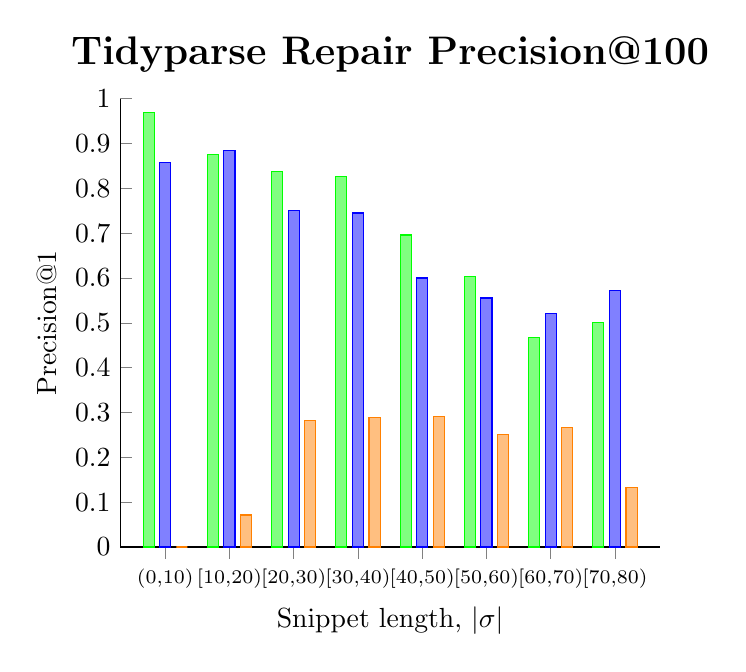
\begin{tikzpicture}
  \begin{axis}[
  xlabel={Snippet length, $|\sigma|$},
  ylabel={Precision@1},
  title={\Large\textbf{Tidyparse Repair Precision@100}},
  ybar,
  axis lines*=left,
  xtick={0, 10, 20, 30, 40, 50, 60, 70},
  ytick={0, 0.1, 0.2, 0.3, 0.4, 0.5, 0.6, 0.7, 0.8, 0.9, 1.0},
  xticklabels={{(}0{,}10{)}, {[}10{,}20{)}, {[}20{,}30{)}, {[}30{,}40{)}, {[}40{,}50{)}, {[}50{,}60{)}, {[}60{,}70{)}, {[}70{,}80{)}},
  x tick label style={font=\scriptsize},
  ymax=1.0,
  ymin=0.0,
  bar width=4pt,
  ]
  \addplot[green, fill=green!50] coordinates { (0, 0.96875) (10, 0.8763440860215054) (20, 0.8366533864541833) (30, 0.8262910798122066) (40, 0.696) (50, 0.6041666666666666) (60, 0.4666666666666667) (70, 0.5) };
  \addplot[blue, fill=blue!50] coordinates { (0, 0.8571428571428571) (10, 0.8842105263157894) (20, 0.75) (30, 0.7450980392156863) (40, 0.6) (50, 0.5555555555555556) (60, 0.52) (70, 0.5714285714285714) };
  \addplot[orange, fill=orange!50] coordinates { (0, 0.0) (10, 0.07142857142857142) (20, 0.28125) (30, 0.2894736842105263) (40, 0.2916666666666667) (50, 0.25) (60, 0.26666666666666666) (70, 0.13333333333333333) };
  \end{axis}
\end{tikzpicture}